% Options here are passed to the article class.
% Most common options: 10pt, 11pt, 12pt
\documentclass[10pt]{datasheet}

% Input encoding and typographical rules for English language
\usepackage[utf8]{inputenc}
\usepackage[english]{babel}
\usepackage[english]{isodate}

% tikz is used to draw images in this example, but you can
% also use \includegraphics{}.
\usepackage{graphicx}
\usepackage{float}
\usepackage{subcaption}

% These define global texts that are used in headers and titles.
\title{DH04: Quad Display Slice With Slider Top Display}
\author{Basil, JayRoi}
\tags{display-halls, quad-display, slice, passive-read}
\date{23 December 2023}
\revision{Revision 2}
\begin{document}
\maketitle

\section{Features}

\begin{itemize}
\item{Fully hopperlocked with local top display locking}
\item{Waterstream inputs}
\item{Passive read restock system with in-slice lists}
\item{Global first box placement}
\end{itemize}

\section{Applications}

\begin{itemize}
\item{Encoded quad-display hall}
\end{itemize}

\section{General Description}
The DH04 quad display slice has 4 box displays with passive read ability. It has a fully hopperlocked layout with no visible pistons. The bottom displays has one buffer box with global first box placement. Box collection is not fully reliable. Top display will break if used aggressively by activating with adjacent slices. Two alternative layouts are available.

\vfill\break

\begin{figure}[H]
    \centering
    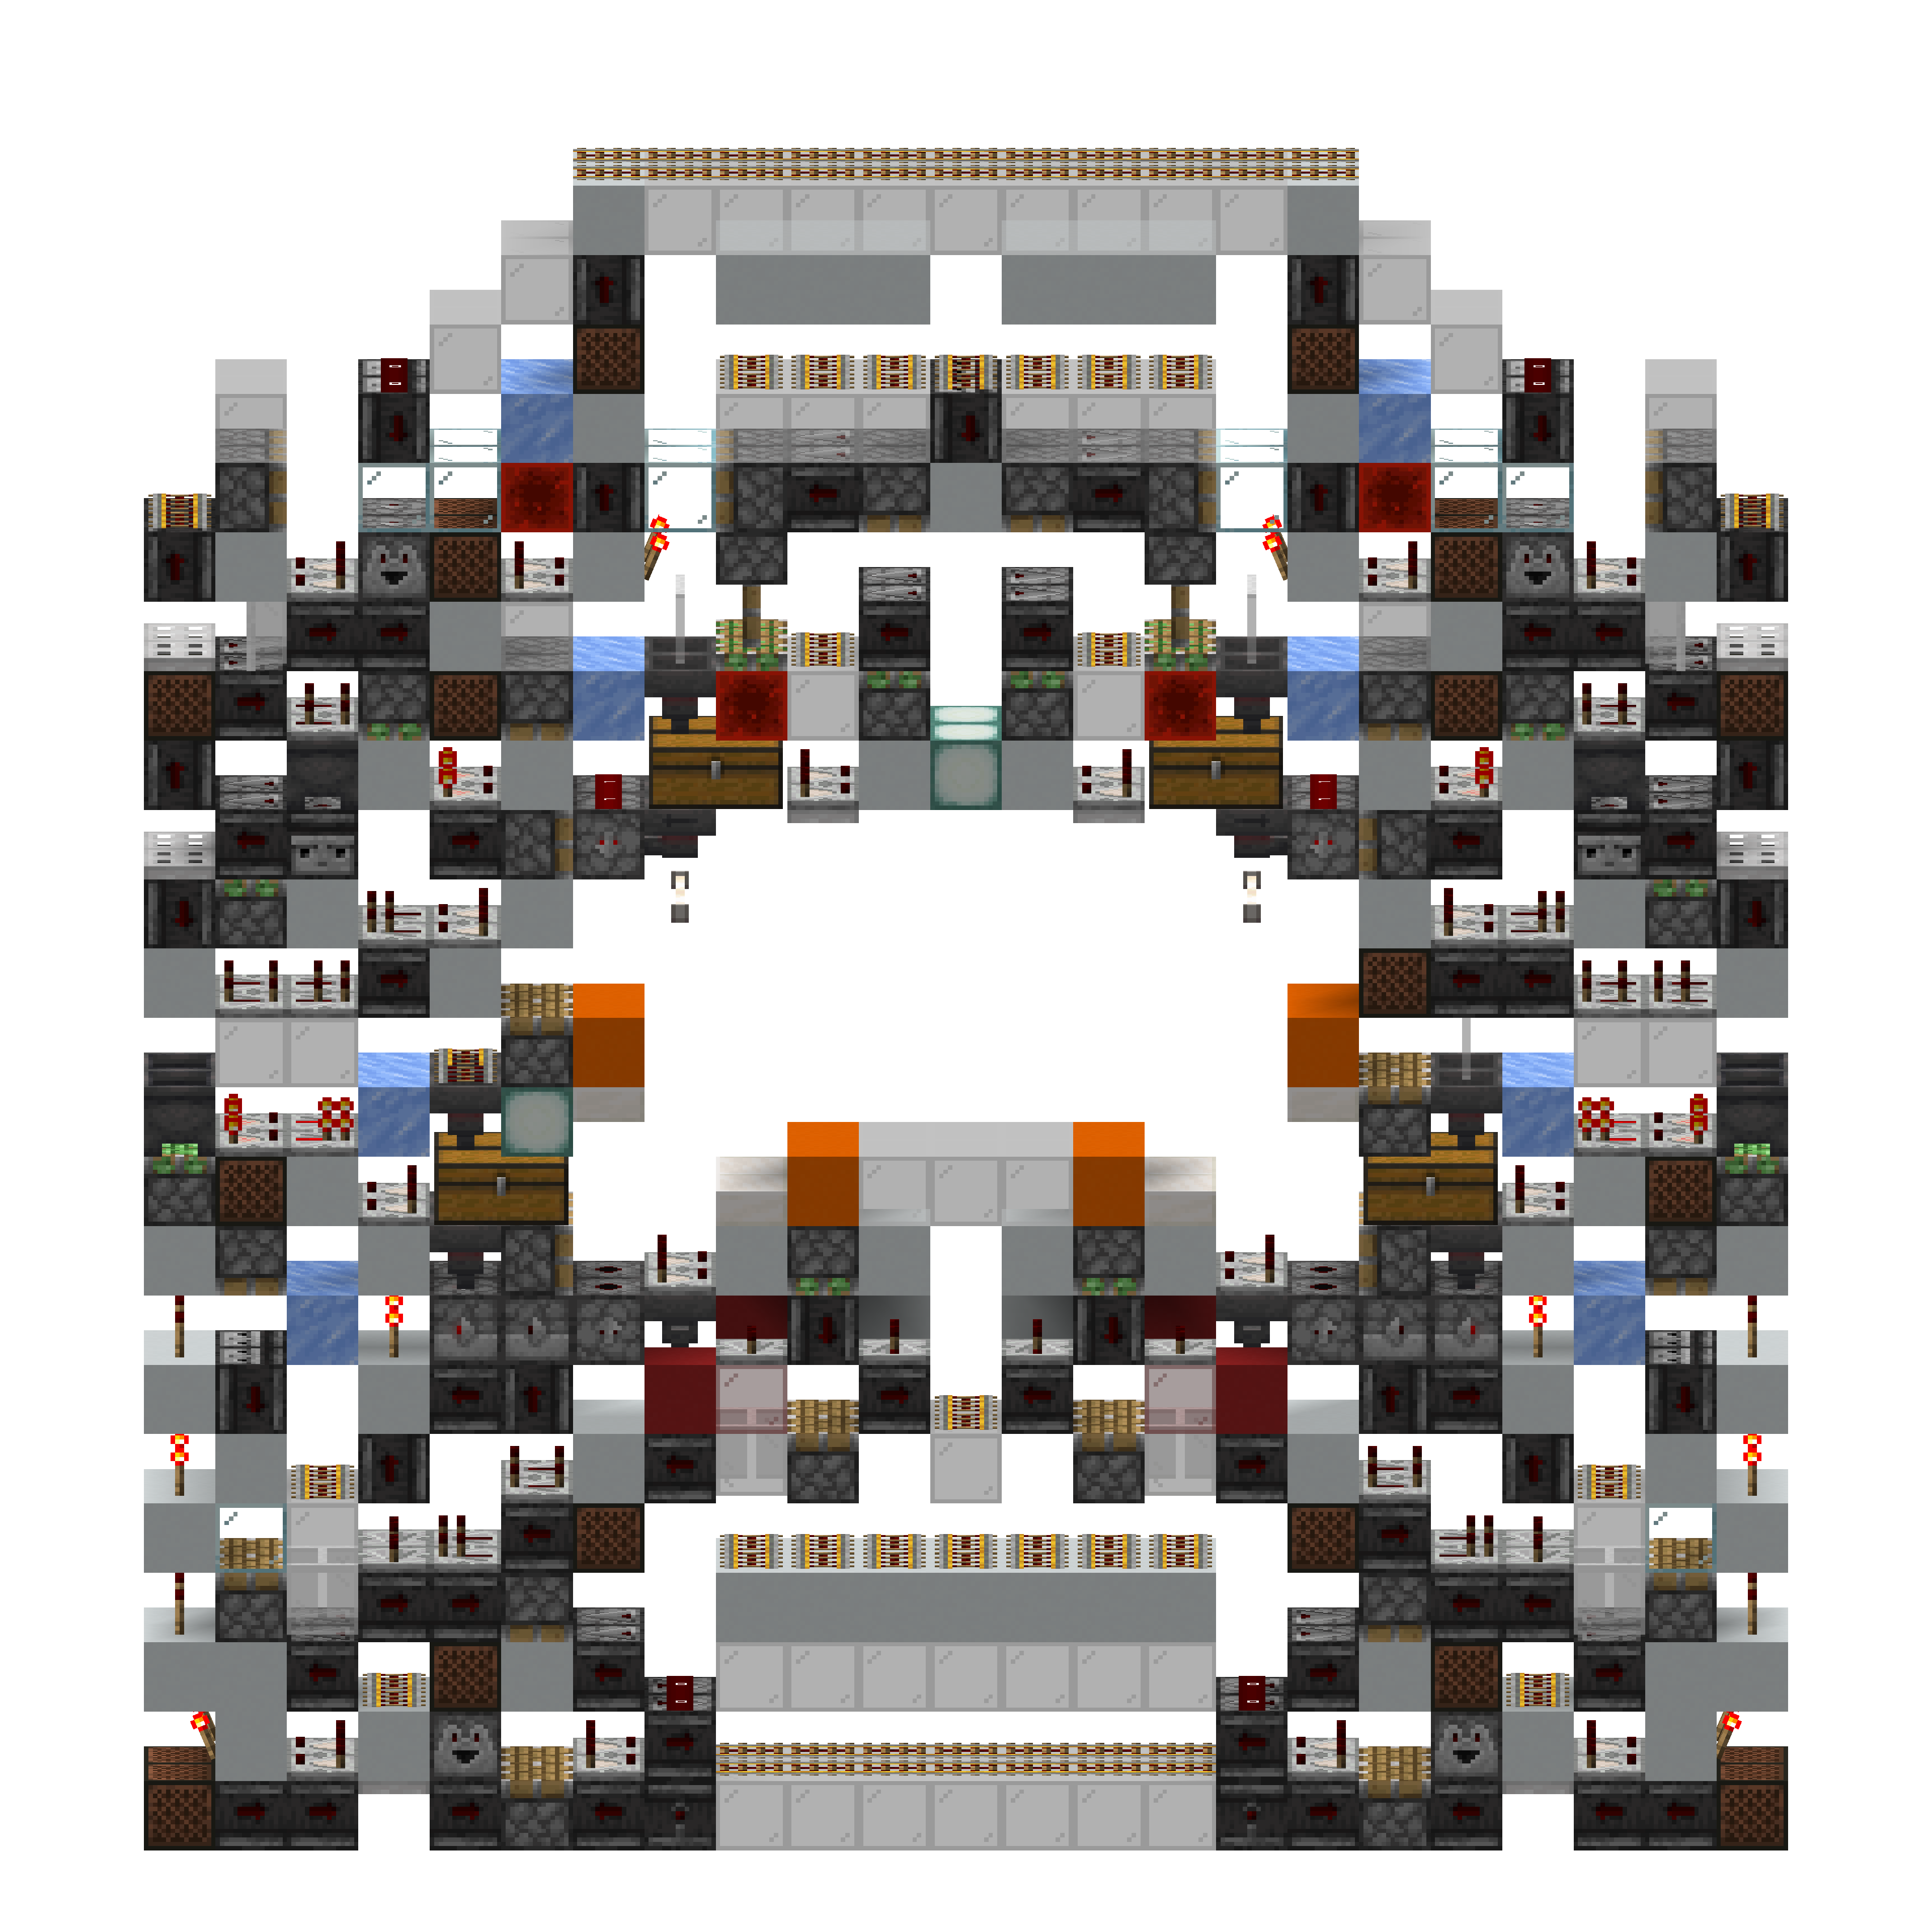
\includegraphics[width=0.48\textwidth]{slice2.png}
    \caption{\centering Quad Display Slice With Slider Top Display}
\end{figure}

% For wide tables, a single column layout is better. It can be switched
% page-by-page.
\onecolumn

\section{Device Specifications}

\begin{table}[H]
    \caption{Device Specifications}
    \begin{tabularx}{\textwidth}{l | c c c | c | X}
        \thickhline
        \textbf{Parameter} & \textbf{Min.} & \textbf{Typ.} & \textbf{Max.} &
        \textbf{Unit} & \textbf{Conditions} \\
        \hline
        Item Throughput  & 8 & - & - & gt & Normal Usage \\
        \hline
        MC Version & 1.13 & 1.19 & - & MCV & Latest version at time of writing: 1.20.4\\
        \hline
        Dimensions & & 2 x 25 x 23 & & Blocks & \\
        \thickhline
\end{tabularx}
\end{table}
\section{Testing Data}
\begin{table}[H]
\caption{Executed Tests}
\begin{tabularx}{\textwidth}{l | X}
    \thickhline
    \textbf{Test} & \textbf{Result} \\
    \hline
    Display operation & Box displays were able to replace boxes when emptied. \\
    \thickhline
\end{tabularx}
\end{table}

\section{Download Information}
\begin{table}[H]
    \caption{Download Information}
    \begin{tabularx}{\textwidth}{l | l | l | X}
        \thickhline
        \textbf{Identifier} & \textbf{MC} & \textbf{File} & \textbf{Description} \\
        \hline
        DH04 & 1.19 & \href{https://github.com/Soontech-Annals/Archive/blob/b56572c0d2b4f182d9e9d41449d8cb2963b923ae/Archive/display-halls/DH04\%20Quad\%20Display\%20Slice\%20With\%20Slider\%20Top\%20Display/DH04\_Quad\_Display\_Slice\_With\_Slider\_Top\_Display.litematic?raw=1}{DH04\_Quad\_Display\_Slice\_With\_Slider\_Top\_Display.litematic} & Schematic of device. Side with rails in waterstream incompatible with MCV \textless 1.17\\
        \hline
        \thickhline
    \end{tabularx}
\end{table}

\end{document}

